%!TEX encoding = UTF-8 Unicode
%!TEX program = xelatex
%% This template licensed under CC-BY-NC-SA by Koenraad De Smedt
\documentclass[final, fmstyle, 12pt]{article}
\usepackage[utf8]{inputenc}
%\usepackage[spanish]{babel}
\usepackage[margin=24mm]{geometry}
\usepackage{fontspec,xltxtra,polyglossia,titling,graphicx,dingbat}
\usepackage{verbatim,gb4e,synttree,multicol} % choose or add what you need   
\usepackage[colorlinks,urlcolor=blue,citecolor=black,linkcolor=black]{hyperref}
\setmainfont[Mapping=tex-text]{Times New Roman} % or another similar font
\setdefaultlanguage{spanish}
%\setotherlanguages{english}
\usepackage[numbers]{natbib}
\usepackage{xspace}
\usepackage{float}
\usepackage{dirtytalk}
\usepackage{subfiles}

\hypersetup{
    colorlinks=true,
    linkcolor=black,
    filecolor=magenta,      
    urlcolor=black,
    pdftitle={Memoria experiencia profesional},
    pdfpagemode=FullScreen,
    }
\urlstyle{same}
\frenchspacing
%\newcommand{\checkmark}{x}

\title{MEMORIA DE EXPERIENCIA PROFESIONAL GRUPO TOMZA}
\author{Héctor Hugo Vidaña Arrieta}
\date{\today}
\hyphenation{unicode}
\usepackage{url}
\usepackage{hyperref}
%\usepackage[bitstream-charter]{mathdesign}
\begin{document}
\renewcommand{\tablename}{Tabla}
	\thispagestyle{empty}
\begin{center} \vfill
{\Large UNIVERSIDAD AUTÓNOMA DE CIUDAD JUÁREZ}\\
\vspace{6mm}
{\large Instituto de Ingeniería y Tecnología\\
\vspace{6mm}
Departamento de Ingeniería Eléctrica y Computación
\vspace{20mm}


\includegraphics [scale=0.7]{Imagenes/escudo-uacj} 
\vspace{10mm}


\thetitle\\
\vspace{15mm}

Protocolo de investigación presentado por:\\
\vspace{6mm}
\theauthor\hspace{10mm} 159957\\
\vspace{10mm}
Requisito para la obtención del título de\\
\vspace{6mm}
INGENIERO EN SOFTWARE\\
\vspace{10mm}

Asesora:\\
{Dra. Julia Patricia Sánchez Solis}\\
} \vfill
	Ciudad Juárez, Chihuahua \hspace{70mm}\today

% {\small \href{https://creativecommons.org/licenses/by/4.0/}{\includegraphics[height=1.2em]{cc-by}} by \theauthor}
\clearpage

\end{center}

\begin{center}

\includegraphics [scale=0.8] {Imagenes/Pdf/firmas1.pdf}
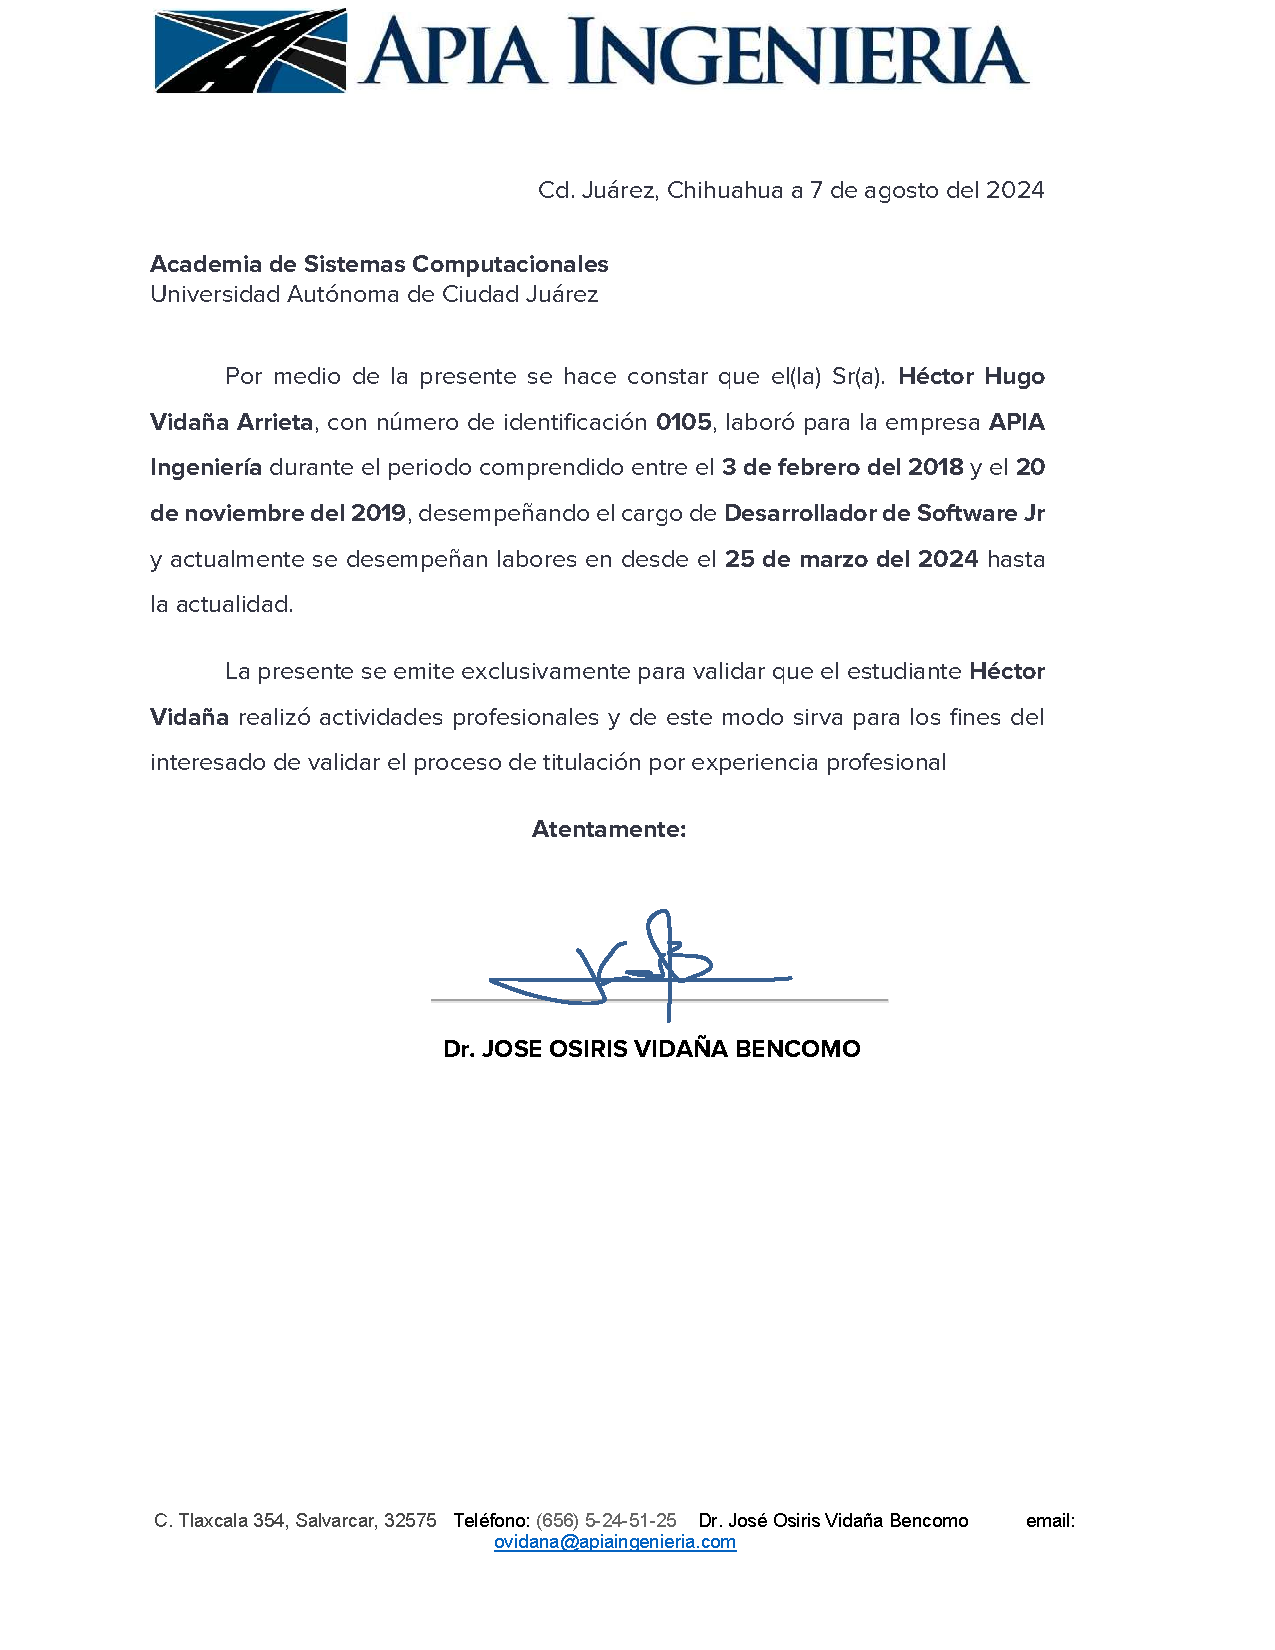
\includegraphics [scale=0.8]
{Imagenes/Pdf/firma2.pdf}
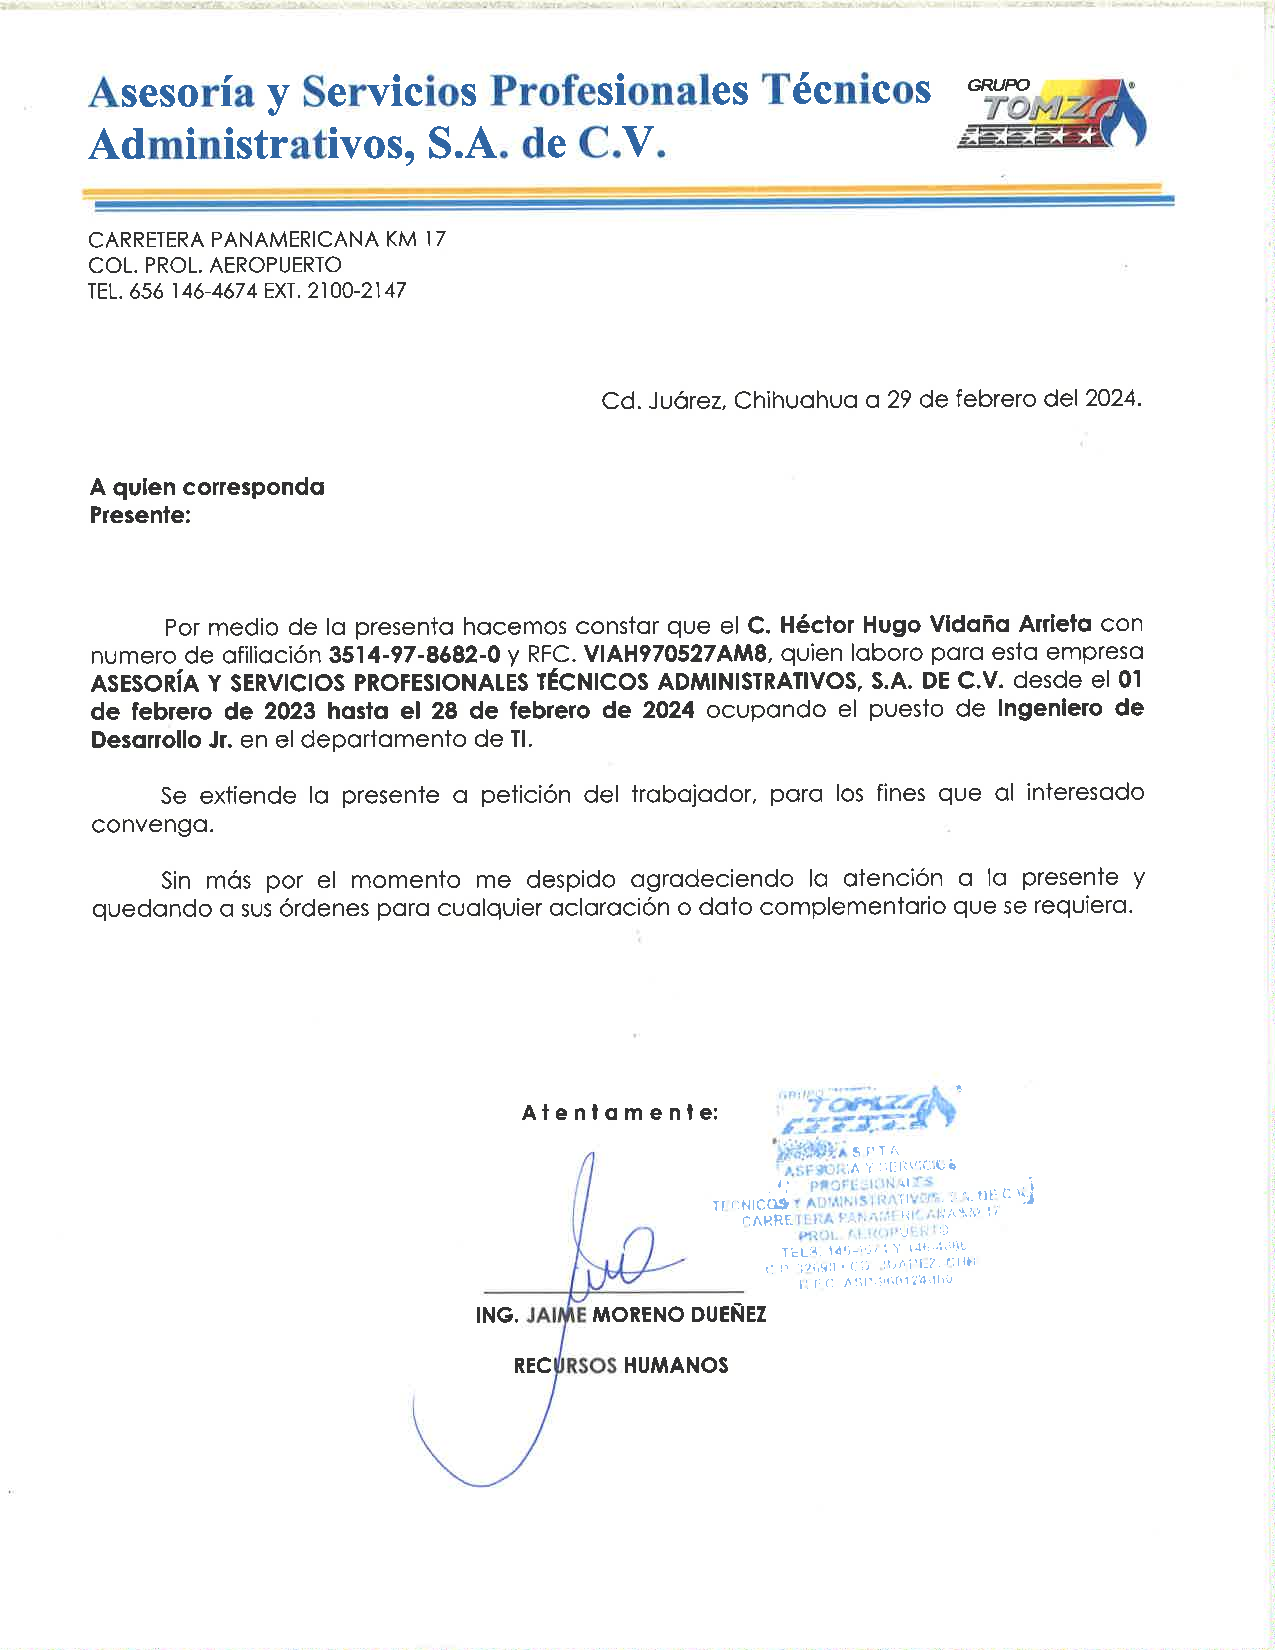
\includegraphics[scale=0.8]{Imagenes/Pdf/firma3.pdf}
\end{center}

\section{Agradecimientos}
\setlength{\parskip}{1em}
En primer lugar, quiero expresar mi más profunda gratitud a mi asesor de tesis, Dra Julia Patricia Sánchez Solis, por su invaluable guía, paciencia y apoyo a lo largo de este proceso. Sus conocimientos, consejos y retroalimentación fueron fundamentales para la culminación de este trabajo.
Agradezco también a los miembros del comité revisor, por su tiempo y dedicación en la evaluación de esta tesis. Sus comentarios y sugerencias contribuyeron significativamente a mejorar la calidad de la investigación.

Extiendo mi agradecimiento a la Universidad Autónoma de Ciudad Juárez (UACJ) y al Instituto de Ingeniería y Tecnología (IIT) por brindarme la oportunidad de formarme como ingeniero en software y por proporcionarme las herramientas y recursos necesarios para llevar a cabo este proyecto.
Un agradecimiento especial a mis profesores del programa de Ingeniería en Software, quienes con su pasión por la enseñanza y su experiencia en el campo me inspiraron y me brindaron las bases para mi desarrollo profesional.

A mis compañeros y amigos, Emmanuel Saldivar Arzaga y Eduardo Ontiveros, gracias por su apoyo, compañerismo y por compartir conmigo esta etapa de aprendizaje y crecimiento.
Finalmente, quiero agradecer a mi familia, en especial a mis padres, María del Carmen Arrieta Serrata y Hector Vidaña Bencomo, por su amor incondicional, su constante apoyo y por creer en mí en cada paso que doy.
A todos ustedes, muchas gracias.


\section{Dedicatoria}
\setlength{\parskip}{1em}
A mis padres, Héctor Vidaña Bencomo y María del Carmen Arrieta Serrata,  mi fuente inagotable de inspiración y apoyo.
A mi padre, Héctor, hombre de carácter recio y corazón noble. Gracias por enseñarme el valor de la disciplina, la importancia de la honestidad y la fuerza de la perseverancia.  Recuerdo tus palabras de aliento en los momentos difíciles y cómo me impulsaste a no rendirme ante los desafíos.  Tu ejemplo de trabajo incansable ha sido mi guía a lo largo de esta travesía.
A mi madre, María del Carmen,  mujer de  amor infinito y  bondad inmensa.  Gracias por ser el pilar de nuestra familia, por tu paciencia y comprensión, por tus noches en vela cuidando mis sueños y por celebrar cada uno de mis logros.  Tu fortaleza y  tu fe inquebrantable me han dado la confianza para perseguir mis metas.
A ambos, gracias por el hogar que con tanto amor construyeron,  por los valores que sembraron en mí, por las enseñanzas que me acompañarán siempre y por el apoyo incondicional que me brindaron a lo largo de mi carrera. Este logro es el resultado de sus esfuerzos,  de sus sacrificios y de su amor infinito.


Con profunda gratitud y admiración.




\section{Introducción}
\setlength{\parskip}{1em} 
El presente documento expone las experiencias profesionales de Héctor Hugo Vidaña Arrieta, 
adquiridas durante su trayectoria laboral en tres empresas del sector tecnológico: 
Grupo Tomza, Apia Ingeniería y Soluciones Móviles y Comunicaciones. 
Empresas que se desenvuelven en el dinámico sector de las tecnologías de la información, 
con un enfoque particular en el desarrollo de software, administración de bases de datos,
sistemas embebidos e inteligencia artificial. Grupo Tomza y Soluciones Móviles se caracteriza por ser empresas consolidadas con una amplia trayectoria en el mercado tecnológico, mientras que Apia Ingeniería es una startup en crecimiento que se destaca por su cultura ágil y flexible.

En este documento se detallarán los proyectos en los que Héctor Hugo Vidaña participó, destacando su relación con las áreas de conocimiento de la ingeniería de software, tales como  desarrollo de software, administración de bases de datos,
sistemas embebidos e inteligencia artificial.  Cada proyecto se describirá a detalle, incluyendo el contexto, los objetivos, las metodologías empleadas y los resultados obtenidos.

A través de la descripción de estas experiencias, se busca ilustrar la aplicación práctica de la formación académica de Héctor Hugo Vidaña Arrieta y cómo ésta contribuyó al desarrollo de su perfil profesional. Se  evidenciará cómo los conocimientos teóricos adquiridos durante sus estudios se complementaron con la experiencia práctica en el campo laboral,  permitiéndole afrontar los desafíos y  contribuir al éxito de los proyectos en los que se involucró.

Finalmente, se presentarán las conclusiones derivadas de estas experiencias, incluyendo una reflexión sobre el impacto de la formación académica en el desempeño profesional,  así como  sugerencias para fortalecer el programa de estudios de la ingeniería de software.
% [Indique de forma clara y coherente en una cuartilla cuál es la nueva contribución, su importancia y por qué es adecuado para sistemas computacionales. Se sugiere para su redacción seguir los cinco pasos siguientes: 1) Establezca el campo de investigación al que pertenece el proyecto, 2) describa los aspectos del problema más que ya han sido estudiado por otros investigadores, 3) explique el área de oportunidad que pretende cubrir el proyecto propuesto, 4) describa el propósito/objetivo del proyecto y 5) proporcione el valor positivo o la justificación para llevar a cabo el proyecto.] 
% \newpage
\newpage
\tableofcontents 

% Entorno Laboral
\newpage 
\subfile{entorno-laboral}

\newpage 
\subfile{experiencia-laboral}

\newpage 
\subfile{Resultados}
\newpage 
\subfile{conclusiones}

\newpage
\bibliographystyle{IEEEtranN}
% \bibliographystyle{plainurl}
\begin{thebibliography}{99}
    \bibitem{obrien2013} O'Brien, J. A., y Marakas, G. M. (2013). \textit{Management Information Systems}. McGraw-Hill Irwin.
    \bibitem{turban2010} Turban, E., Sharda, R., Delen, D., y King, D. (2010). \textit{Business intelligence: A managerial approach}. Pearson Education.
    \bibitem{russell2010} Russell, S. J., y Norvig, P. (2010). \textit{Artificial Intelligence: A Modern Approach}. Pearson Education.
\end{thebibliography}
%\nocite{*} 

\section{Apéndice}
\begin{center}
    
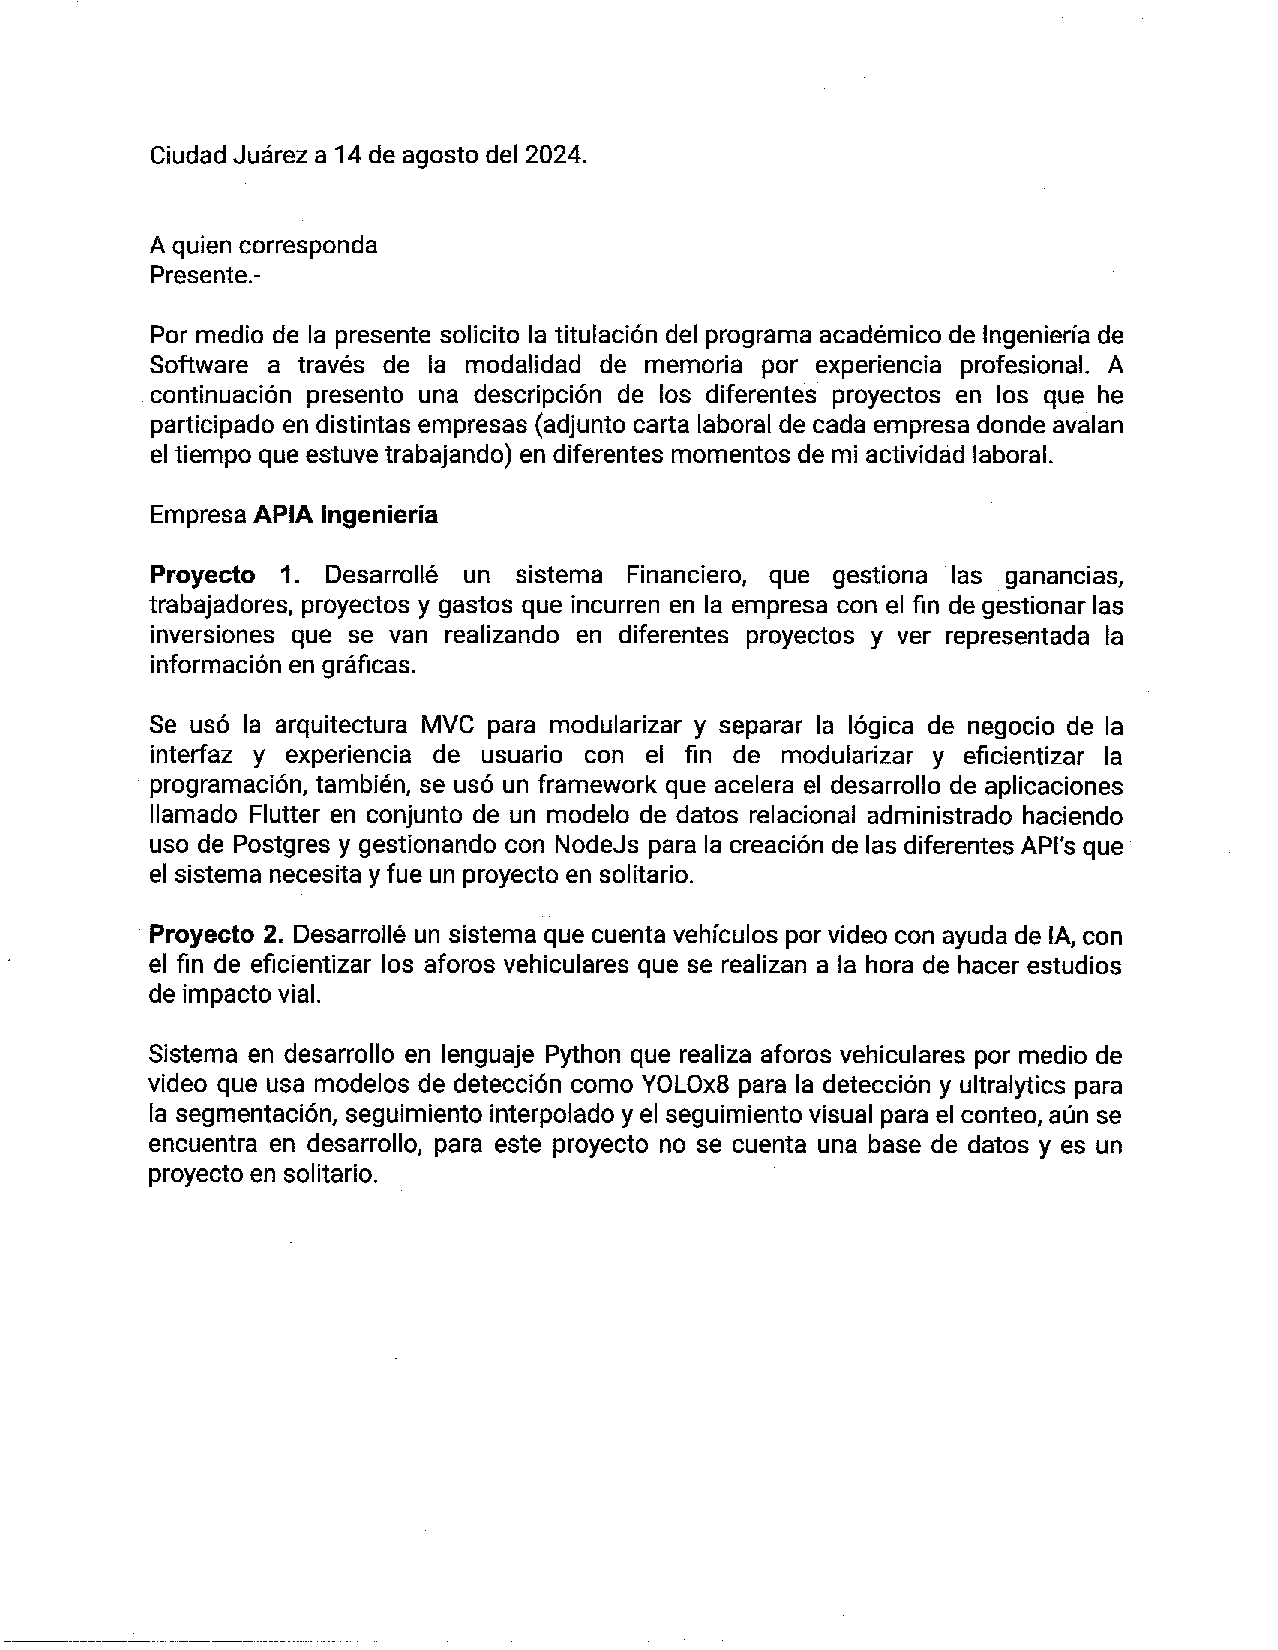
\includegraphics[scale=0.8]{Imagenes/Pdf/Carta1.pdf}

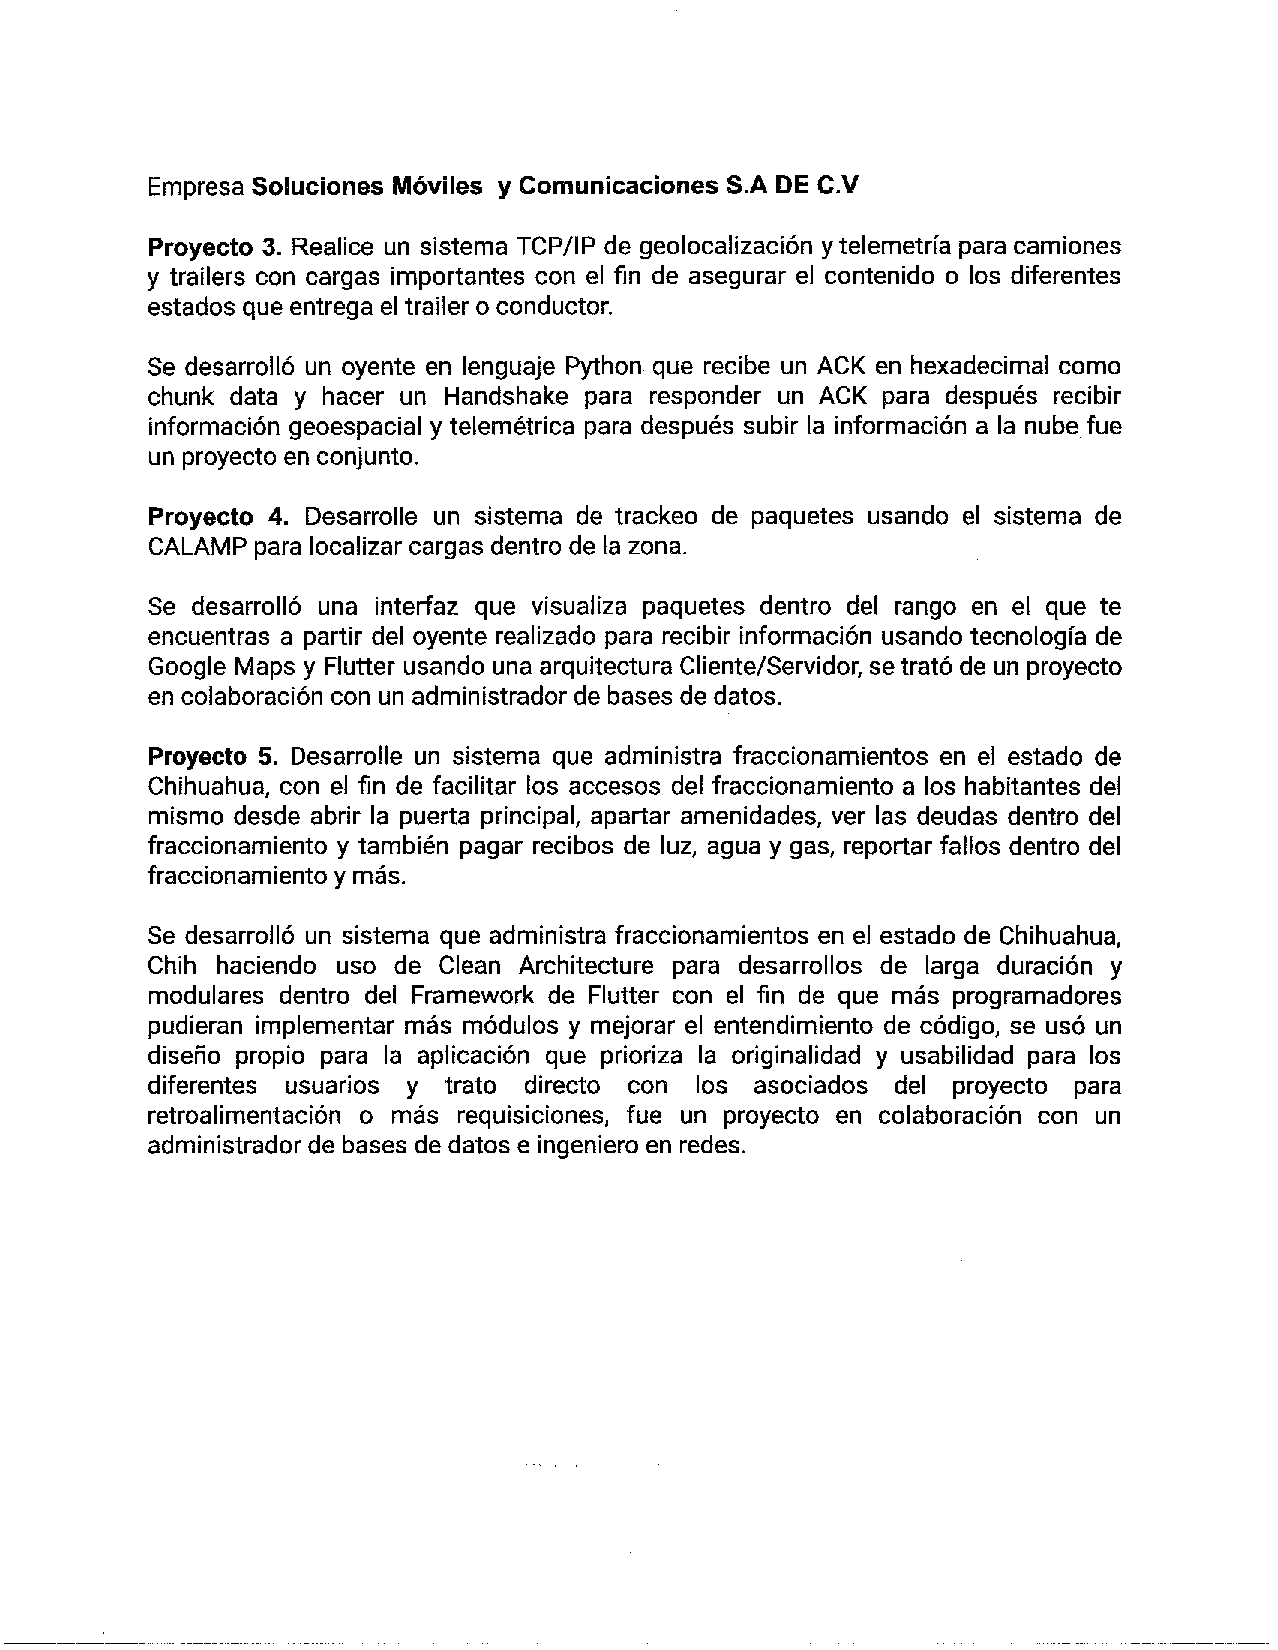
\includegraphics[scale=0.8]{Imagenes/Pdf/Carta2.pdf}

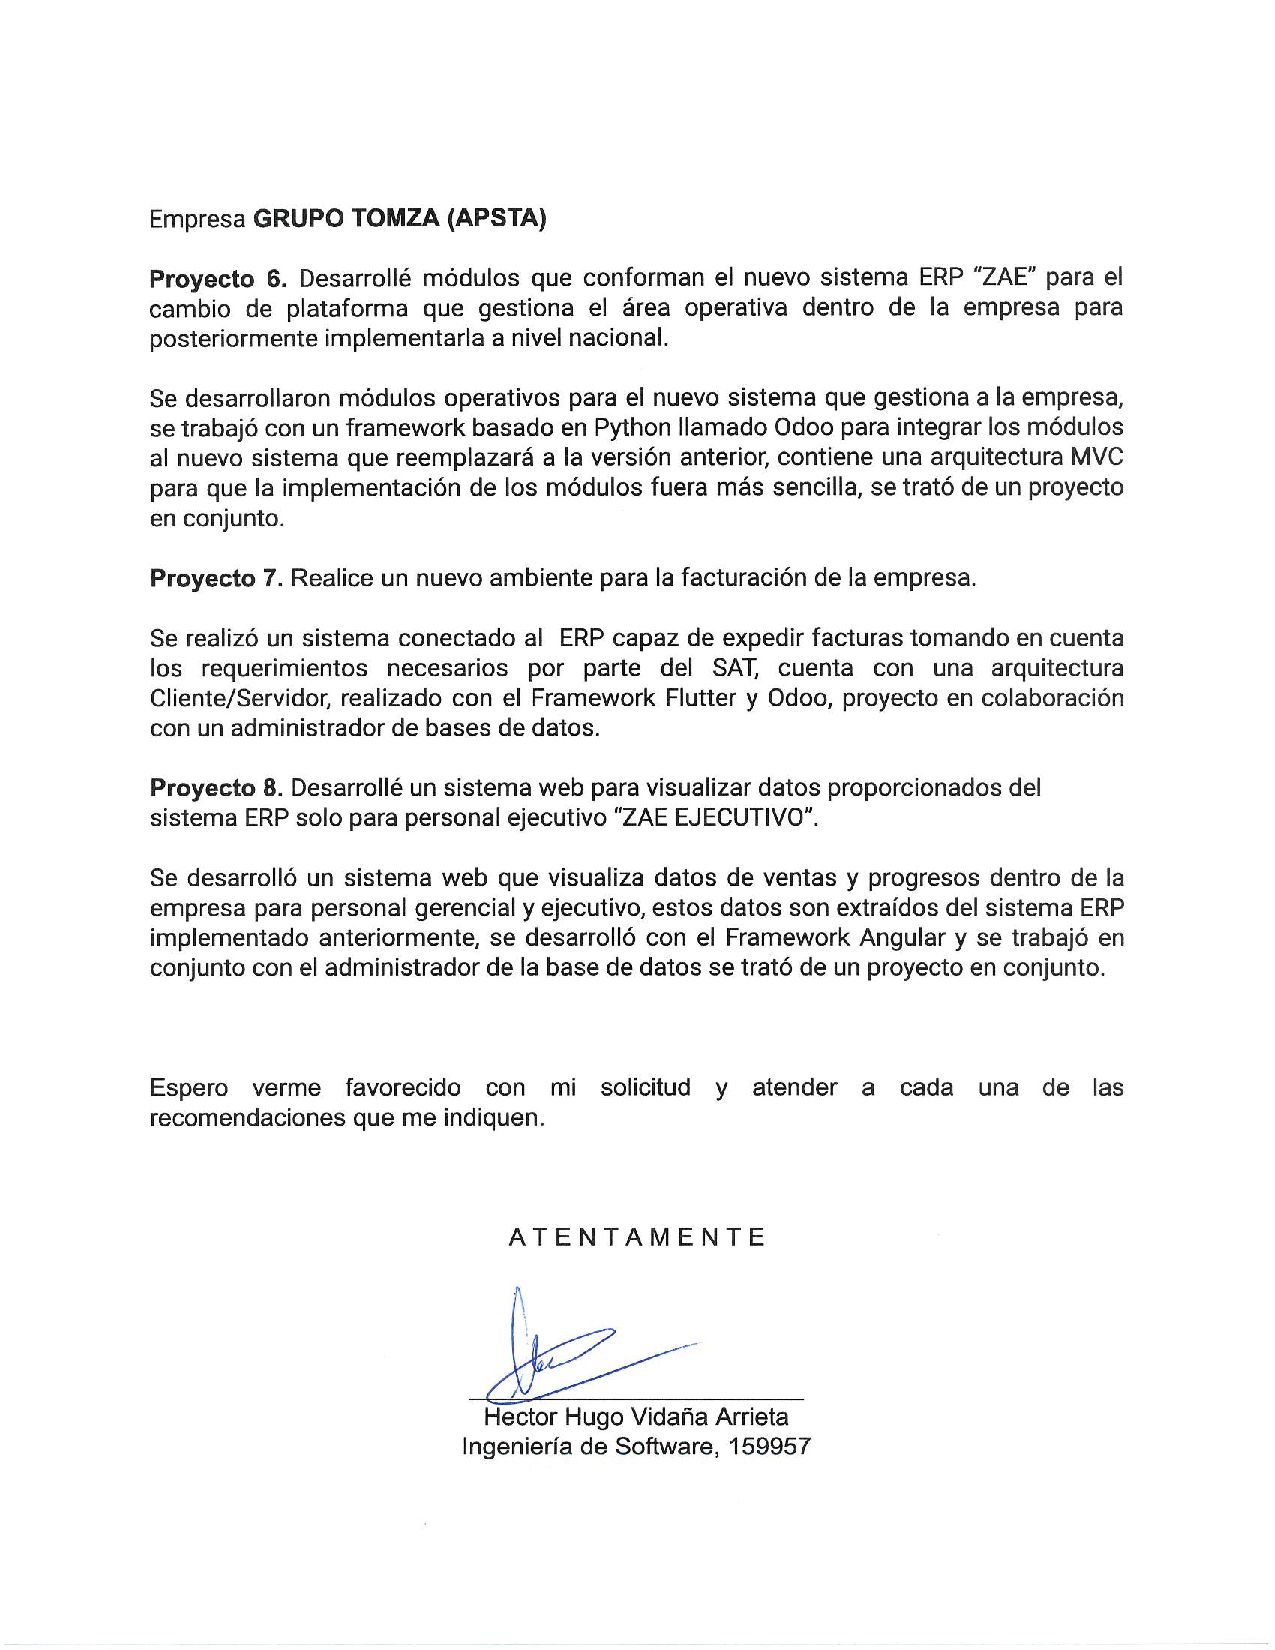
\includegraphics[scale=0.8]{Imagenes/Pdf/Carta3.pdf}

\end{center}

\end{document}  